\documentclass{article}
% generated by Madoko, version 1.1.6
%mdk-data-line={1}


\usepackage[heading-base={2},section-num={False},bib-label={hide},fontspec={True}]{madoko2}
\usepackage{float}


\begin{document}



%mdk-data-line={8}
\mdxtitleblockstart{}
%mdk-data-line={8}
\mdxtitle{\mdline{8}The Second Day}%mdk
\mdxauthorstart{}
%mdk-data-line={13}
\mdxauthorname{\mdline{13}22 January 2019}%mdk
\mdxauthorend\mdtitleauthorrunning{}{}\mdxtitleblockend%mdk
\mdline{10}
\begin{mdtoc}%mdk

\section*{Contents}\label{sec-contents}%mdk%mdk

\begin{mdtocblock}%mdk

\mdtocitemx{sec-session-two}{\mdref{sec-session-two}{1.\hspace*{0.5em}Session Two}}%mdk

\begin{mdtocblock}%mdk

\mdtocitemx{sec-testing-wavelengths}{\mdref{sec-testing-wavelengths}{1.1.\hspace*{0.5em}Testing Wavelengths}}%mdk

\begin{mdtocblock}%mdk

\mdtocitemx{sec-procedure-practical-method}{\mdref{sec-procedure-practical-method}{1.1.1.\hspace*{0.5em}Procedure (Practical Method)}}%mdk

\mdtocitemx{sec-evaluation-of-procedure}{\mdref{sec-evaluation-of-procedure}{1.1.2.\hspace*{0.5em}Evaluation of Procedure}}%mdk

\mdtocitemx{sec-table-of-results}{\mdref{sec-table-of-results}{1.1.3.\hspace*{0.5em}Table of Results.}}%mdk

\mdtocitemx{sec-evaluation-of-readings}{\mdref{sec-evaluation-of-readings}{1.1.4.\hspace*{0.5em}Evaluation of Readings}}%mdk

\mdtocitemx{sec-analysis-of-readings}{\mdref{sec-analysis-of-readings}{1.1.5.\hspace*{0.5em}Analysis of Readings}}%mdk
%mdk
\end{mdtocblock}%mdk
%mdk
\end{mdtocblock}%mdk
%mdk
\end{mdtocblock}%mdk
%mdk
\end{mdtoc}%mdk

%mdk-data-line={12}
\section{\mdline{12}1.\hspace*{0.5em}\mdline{12}Session Two}\label{sec-session-two}%mdk%mdk

%mdk-data-line={13}
\subsection{\mdline{13}1.1.\hspace*{0.5em}\mdline{13}Testing Wavelengths}\label{sec-testing-wavelengths}%mdk%mdk

%mdk-data-line={16}
\subsubsection{\mdline{16}1.1.1.\hspace*{0.5em}\mdline{16}Procedure (Practical Method)}\label{sec-procedure-practical-method}%mdk%mdk

%mdk-data-line={18}
\begin{enumerate}[noitemsep,topsep=\mdcompacttopsep]%mdk

%mdk-data-line={18}
\item\mdline{18}Set up the equipment with colored LEDs and two filters.%mdk

%mdk-data-line={19}
\item\mdline{19}Turn on the microcontroller, and set the filters to a 0 degrees offset.%mdk

%mdk-data-line={20}
\item\mdline{20}Record the initial intensity sensor value.%mdk

%mdk-data-line={21}
\item\mdline{21}Change the angle between the two filters in steps of 5 degrees, and record the intensity sensor value at each offset interval, being careful not to misalign the sensor or LED.%mdk

%mdk-data-line={22}
\item\mdline{22}Repeat steps 3 and 4 until a sufficient number of repeats has been obtained to reduce the impact of anomalous results.%mdk

%mdk-data-line={23}
\item\mdline{23}Repeat steps with different colors of LEDs: Red, Green, and Blue%mdk
%mdk
\end{enumerate}%mdk

%mdk-data-line={25}
\subsubsection{\mdline{25}1.1.2.\hspace*{0.5em}\mdline{25}Evaluation of Procedure}\label{sec-evaluation-of-procedure}%mdk%mdk

%mdk-data-line={27}
\noindent\mdline{27}This procedure was relatively easy, as I could use the same set-up as experiment 1. The major issue encountered was the variation in initial intensity. With experiment 1, only one type LED was used, so each repeat started with roughly the same initial conditions. With this experiment, each LED had a different initial brightness, as can be observed in the results below. This, however, will not affect my results, as I can both account for this in the final analysis, and compare each set of data separately.%mdk

%mdk-data-line={29}
\subsubsection{\mdline{29}1.1.3.\hspace*{0.5em}\mdline{29}Table of Results.}\label{sec-table-of-results}%mdk%mdk

%mdk-data-line={31}
\begin{table}[H]%mdk
\begin{mdcenter}%mdk
\begin{mdtabular}{6}{\dimeval{(\linewidth)/6}}{1ex}%mdk
\begin{tabular}{lccccc}\cmidrule[\dimpx{2}]{2-2}\cmidrule[\dimpx{2}]{3-3}\cmidrule[\dimpx{2}]{4-4}\cmidrule[\dimpx{2}]{5-5}\cmidrule[\dimpx{2}]{6-6}
{\mdseries\mdline{33}Angle}&{\mdseries\mdline{33} Raw sensor output}&{\mdseries\mdline{33}}&{\mdseries\mdline{33}}&{\mdseries\mdline{33}}&{\mdseries\mdline{33}}\\
{\mdseries\mdline{34}}&{\mdseries\mdline{34} Repeat one}&{\mdseries\mdline{34} Repeat two}&{\mdseries\mdline{34} Repeat three}&{\mdseries\mdline{34} Average}&{\mdseries\mdline{34} Std Dev}\\

\midrule
\mdline{36} 0&\mdline{36} 162&\mdline{36} 178&\mdline{36} 156&\mdline{36} 165.3&\mdline{36} 11.4\\
\mdline{37} 5&\mdline{37} 159&\mdline{37} 175&\mdline{37} 157&\mdline{37} 163.7&\mdline{37} 9.9\\
\mdline{38} 10&\mdline{38} 151&\mdline{38} 168&\mdline{38} 157&\mdline{38} 157.0&\mdline{38} 9.5\\
\mdline{39} 15&\mdline{39} 145&\mdline{39} 160&\mdline{39} 148&\mdline{39} 151.0&\mdline{39} 7.9\\
\mdline{40} 20&\mdline{40} 136&\mdline{40} 155&\mdline{40} 139&\mdline{40} 143.3&\mdline{40} 10.2\\
\mdline{41} 25&\mdline{41} 124&\mdline{41} 141&\mdline{41} 131&\mdline{41} 132.0&\mdline{41} 8.5\\
\mdline{42} 30&\mdline{42} 114&\mdline{42} 124&\mdline{42} 123&\mdline{42} 120.3&\mdline{42} 5.5\\
\mdline{43} 35&\mdline{43} 99&\mdline{43} 111&\mdline{43} 106&\mdline{43} 105.3&\mdline{43} 6.0\\
\mdline{44} 40&\mdline{44} 86&\mdline{44} 95&\mdline{44} 93&\mdline{44} 91.3&\mdline{44} 4.7\\
\mdline{45} 45&\mdline{45} 71&\mdline{45} 81&\mdline{45} 81&\mdline{45} 77.7&\mdline{45} 5.8\\
\mdline{46} 50&\mdline{46} 60&\mdline{46} 69&\mdline{46} 67&\mdline{46} 65.3&\mdline{46} 4.7\\
\mdline{47} 55&\mdline{47} 46&\mdline{47} 52&\mdline{47} 55&\mdline{47} 51.0&\mdline{47} 4.6\\
\mdline{48} 60&\mdline{48} 33&\mdline{48} 39&\mdline{48} 40&\mdline{48} 37.3&\mdline{48} 3.8\\
\mdline{49} 65&\mdline{49} 25&\mdline{49} 28&\mdline{49} 31&\mdline{49} 28.0&\mdline{49} 3.0\\
\mdline{50} 70&\mdline{50} 15&\mdline{50} 16&\mdline{50} 22&\mdline{50} 17.7&\mdline{50} 3.8\\
\mdline{51} 75&\mdline{51} 10&\mdline{51} 9&\mdline{51} 14&\mdline{51} 11.0&\mdline{51} 2.6\\
\mdline{52} 80&\mdline{52} 5&\mdline{52} 5&\mdline{52} 7&\mdline{52} 5.6&\mdline{52} 1.2\\
\mdline{53} 85&\mdline{53} 1&\mdline{53} 1&\mdline{53} 2&\mdline{53} 1.3&\mdline{53} 0.6\\
\mdline{54} 90&\mdline{54} 0&\mdline{54} 0&\mdline{54} 0&\mdline{54} 0&\mdline{54} 0\\
\midrule[\dimpx{2}]
\end{tabular}\end{mdtabular}

%mdk-data-line={57}
\mdhr{}%mdk

%mdk-data-line={58}
\noindent\mdline{58}\mdcaption{\textbf{Table~\mdcaptionlabel{1}.}~\mdcaptiontext{Experiment 2: Green LED}}%mdk
%mdk
\end{mdcenter}\label{results}%mdk
%mdk
\end{table}%mdk

%mdk-data-line={59}
\begin{table}[H]%mdk
\begin{mdcenter}%mdk
\begin{mdtabular}{6}{\dimeval{(\linewidth)/6}}{1ex}%mdk
\begin{tabular}{lccccc}\cmidrule[\dimpx{2}]{2-2}\cmidrule[\dimpx{2}]{3-3}\cmidrule[\dimpx{2}]{4-4}\cmidrule[\dimpx{2}]{5-5}\cmidrule[\dimpx{2}]{6-6}
{\mdseries\mdline{61}Angle}&{\mdseries\mdline{61} Raw sensor output}&{\mdseries\mdline{61}}&{\mdseries\mdline{61}}&{\mdseries\mdline{61}}&{\mdseries\mdline{61}}\\
{\mdseries\mdline{62}}&{\mdseries\mdline{62} Repeat one}&{\mdseries\mdline{62} Repeat two}&{\mdseries\mdline{62} Repeat three}&{\mdseries\mdline{62} Average}&{\mdseries\mdline{62} Std Dev}\\

\midrule
\mdline{64} 0&\mdline{64} 275&\mdline{64} 401&\mdline{64} 469&\mdline{64} 381.7&\mdline{64} 98.4\\
\mdline{65} 5&\mdline{65} 273&\mdline{65} 399&\mdline{65} 463&\mdline{65} 378.3&\mdline{65} 96.7\\
\mdline{66} 10&\mdline{66} 268&\mdline{66} 395&\mdline{66} 451&\mdline{66} 371.3&\mdline{66} 93.8\\
\mdline{67} 15&\mdline{67} 263&\mdline{67} 375&\mdline{67} 435&\mdline{67} 357.7&\mdline{67} 87.3\\
\mdline{68} 20&\mdline{68} 241&\mdline{68} 364&\mdline{68} 409&\mdline{68} 338.0&\mdline{68} 87.0\\
\mdline{69} 25&\mdline{69} 222&\mdline{69} 344&\mdline{69} 376&\mdline{69} 314.0&\mdline{69} 81.3\\
\mdline{70} 30&\mdline{70} 206&\mdline{70} 315&\mdline{70} 351&\mdline{70} 290.7&\mdline{70} 75.5\\
\mdline{71} 35&\mdline{71} 182&\mdline{71} 282&\mdline{71} 308&\mdline{71} 257.3&\mdline{71} 66.5\\
\mdline{72} 40&\mdline{72} 152&\mdline{72} 252&\mdline{72} 260&\mdline{72} 221.3&\mdline{72} 60.2\\
\mdline{73} 45&\mdline{73} 113&\mdline{73} 221&\mdline{73} 232&\mdline{73} 195.3&\mdline{73} 54.3\\
\mdline{74} 50&\mdline{74} 110&\mdline{74} 175&\mdline{74} 194&\mdline{74} 159.7&\mdline{74} 44.0\\
\mdline{75} 55&\mdline{75} 86&\mdline{75} 147&\mdline{75} 165&\mdline{75} 132.7&\mdline{75} 41.4\\
\mdline{76} 60&\mdline{76} 64&\mdline{76} 114&\mdline{76} 119&\mdline{76} 99.0&\mdline{76} 30.4\\
\mdline{77} 65&\mdline{77} 46&\mdline{77} 79&\mdline{77} 87&\mdline{77} 70.7&\mdline{77} 21.7\\
\mdline{78} 70&\mdline{78} 32&\mdline{78} 47&\mdline{78} 57&\mdline{78} 45.3&\mdline{78} 12.6\\
\mdline{79} 75&\mdline{79} 12&\mdline{79} 29&\mdline{79} 35&\mdline{79} 25.3&\mdline{79} 11.9\\
\mdline{80} 80&\mdline{80} 6&\mdline{80} 13&\mdline{80} 17&\mdline{80} 12.0&\mdline{80} 5.6\\
\mdline{81} 85&\mdline{81} 2&\mdline{81} 5&\mdline{81} 5&\mdline{81} 4.0&\mdline{81} 1.7\\
\mdline{82} 90&\mdline{82} 0&\mdline{82} 1&\mdline{82} 0&\mdline{82} 0.3&\mdline{82} 0.6\\
\midrule[\dimpx{2}]
\end{tabular}\end{mdtabular}

%mdk-data-line={85}
\mdhr{}%mdk

%mdk-data-line={86}
\noindent\mdline{86}\mdcaption{\textbf{Table~\mdcaptionlabel{2}.}~\mdcaptiontext{Experiment 2: Blue LED}}%mdk
%mdk
\end{mdcenter}\label{results}%mdk
%mdk
\end{table}%mdk

%mdk-data-line={87}
\begin{table}[H]%mdk
\begin{mdcenter}%mdk
\begin{mdtabular}{6}{\dimeval{(\linewidth)/6}}{1ex}%mdk
\begin{tabular}{lccccc}\cmidrule[\dimpx{2}]{2-2}\cmidrule[\dimpx{2}]{3-3}\cmidrule[\dimpx{2}]{4-4}\cmidrule[\dimpx{2}]{5-5}\cmidrule[\dimpx{2}]{6-6}
{\mdseries\mdline{89}Angle}&{\mdseries\mdline{89} Raw sensor output}&{\mdseries\mdline{89}}&{\mdseries\mdline{89}}&{\mdseries\mdline{89}}&{\mdseries\mdline{89}}\\
{\mdseries\mdline{90}}&{\mdseries\mdline{90} Repeat one}&{\mdseries\mdline{90} Repeat two}&{\mdseries\mdline{90} Repeat three}&{\mdseries\mdline{90} Average}&{\mdseries\mdline{90} Std Dev}\\

\midrule
\mdline{92} 0&\mdline{92} 211&\mdline{92} 189&\mdline{92} 198&\mdline{92} 199.3&\mdline{92} 11.1\\
\mdline{93} 5&\mdline{93} 205&\mdline{93} 184&\mdline{93} 186&\mdline{93} 191.7&\mdline{93} 11.6\\
\mdline{94} 10&\mdline{94} 198&\mdline{94} 180&\mdline{94} 181&\mdline{94} 186.3&\mdline{94} 10.1\\
\mdline{95} 15&\mdline{95} 188&\mdline{95} 175&\mdline{95} 177&\mdline{95} 180.0&\mdline{95} 7.0\\
\mdline{96} 20&\mdline{96} 178&\mdline{96} 168&\mdline{96} 166&\mdline{96} 170.7&\mdline{96} 6.4\\
\mdline{97} 25&\mdline{97} 167&\mdline{97} 155&\mdline{97} 157&\mdline{97} 159.7&\mdline{97} 6.4\\
\mdline{98} 30&\mdline{98} 155&\mdline{98} 137&\mdline{98} 141&\mdline{98} 144.3&\mdline{98} 9.5\\
\mdline{99} 35&\mdline{99} 138&\mdline{99} 121&\mdline{99} 123&\mdline{99} 127.3&\mdline{99} 9.3\\
\mdline{100} 40&\mdline{100} 123&\mdline{100} 110&\mdline{100} 110&\mdline{100} 114.3&\mdline{100} 7.5\\
\mdline{101} 45&\mdline{101} 114&\mdline{101} 106&\mdline{101} 104&\mdline{101} 108.0&\mdline{101} 5.3\\
\mdline{102} 50&\mdline{102} 96&\mdline{102} 89&\mdline{102} 92&\mdline{102} 92.3&\mdline{102} 3.5\\
\mdline{103} 55&\mdline{103} 79&\mdline{103} 71&\mdline{103} 69&\mdline{103} 73.0&\mdline{103} 5.3\\
\mdline{104} 60&\mdline{104} 65&\mdline{104} 59&\mdline{104} 59&\mdline{104} 61.0&\mdline{104} 3.5\\
\mdline{105} 65&\mdline{105} 49&\mdline{105} 46&\mdline{105} 47&\mdline{105} 47.3&\mdline{105} 1.5\\
\mdline{106} 70&\mdline{106} 38&\mdline{106} 38&\mdline{106} 39&\mdline{106} 38.3&\mdline{106} 0.6\\
\mdline{107} 75&\mdline{107} 28&\mdline{107} 29&\mdline{107} 29&\mdline{107} 28.7&\mdline{107} 0.6\\
\mdline{108} 80&\mdline{108} 20&\mdline{108} 25&\mdline{108} 22&\mdline{108} 22.3&\mdline{108} 2.5\\
\mdline{109} 85&\mdline{109} 16&\mdline{109} 19&\mdline{109} 18&\mdline{109} 17.7&\mdline{109} 1.5\\
\mdline{110} 90&\mdline{110} 13&\mdline{110} 14&\mdline{110} 12&\mdline{110} 13.0&\mdline{110} 1.0\\
\midrule[\dimpx{2}]
\end{tabular}\end{mdtabular}

%mdk-data-line={113}
\mdhr{}%mdk

%mdk-data-line={114}
\noindent\mdline{114}\mdcaption{\textbf{Table~\mdcaptionlabel{3}.}~\mdcaptiontext{Experiment 2: Red LED}}%mdk
%mdk
\end{mdcenter}\label{results}%mdk
%mdk
\end{table}%mdk

%mdk-data-line={116}
\subsubsection{\mdline{116}1.1.4.\hspace*{0.5em}\mdline{116}Evaluation of Readings}\label{sec-evaluation-of-readings}%mdk%mdk

%mdk-data-line={118}
\noindent\mdline{118}These readings were somewhat harder to achieve than the first experiment. For the green and blue LEDs, the type of LED (10mm) was used, so the results were similar, however with both having noticeably lower initial intensities. This is due to the neutral density effect of the LED coloring, and will not affect my analysis, as we will not need to compare the initial intensity of the different colors directly.%mdk

%mdk-data-line={120}
\mdline{120}The accuracy and standard deviation of these results was somewhat unexpected. The blue LED had error ranges between repeats comparable to the first experiment, but the red and green LEDs both had much smaller deviation between repeats. This is due to the overall intensities being lower, which means that there is a narrower range of results, due to the resolution of the sensor being 1.%mdk

%mdk-data-line={122}
\subsubsection{\mdline{122}1.1.5.\hspace*{0.5em}\mdline{122}Analysis of Readings}\label{sec-analysis-of-readings}%mdk%mdk

%mdk-data-line={124}
\noindent\mdline{124}We can make the same substitutions as Experiment one to verify that these results follow Malus\mdline{124}'\mdline{124}s law, with wavelength having no effect:%mdk

%mdk-data-line={126}
\mdline{126}$I\propto\cos^2\theta$\mdline{126}%mdk

%mdk-data-line={128}
\mdline{128}$I=I_0\cos^2\theta$\mdline{128}%mdk

%mdk-data-line={130}
\mdline{130}$\Rightarrow y=mx+c$\mdline{130}%mdk

%mdk-data-line={132}
\mdline{132}$\therefore y=I, m=I_0, x=\cos^2\theta, c=0$\mdline{132}%mdk

%mdk-data-line={134}
\mdline{134}These were then plotted as a line graph for each color, and lines of best fit were generated:%mdk

%mdk-data-line={136}
\mdline{136}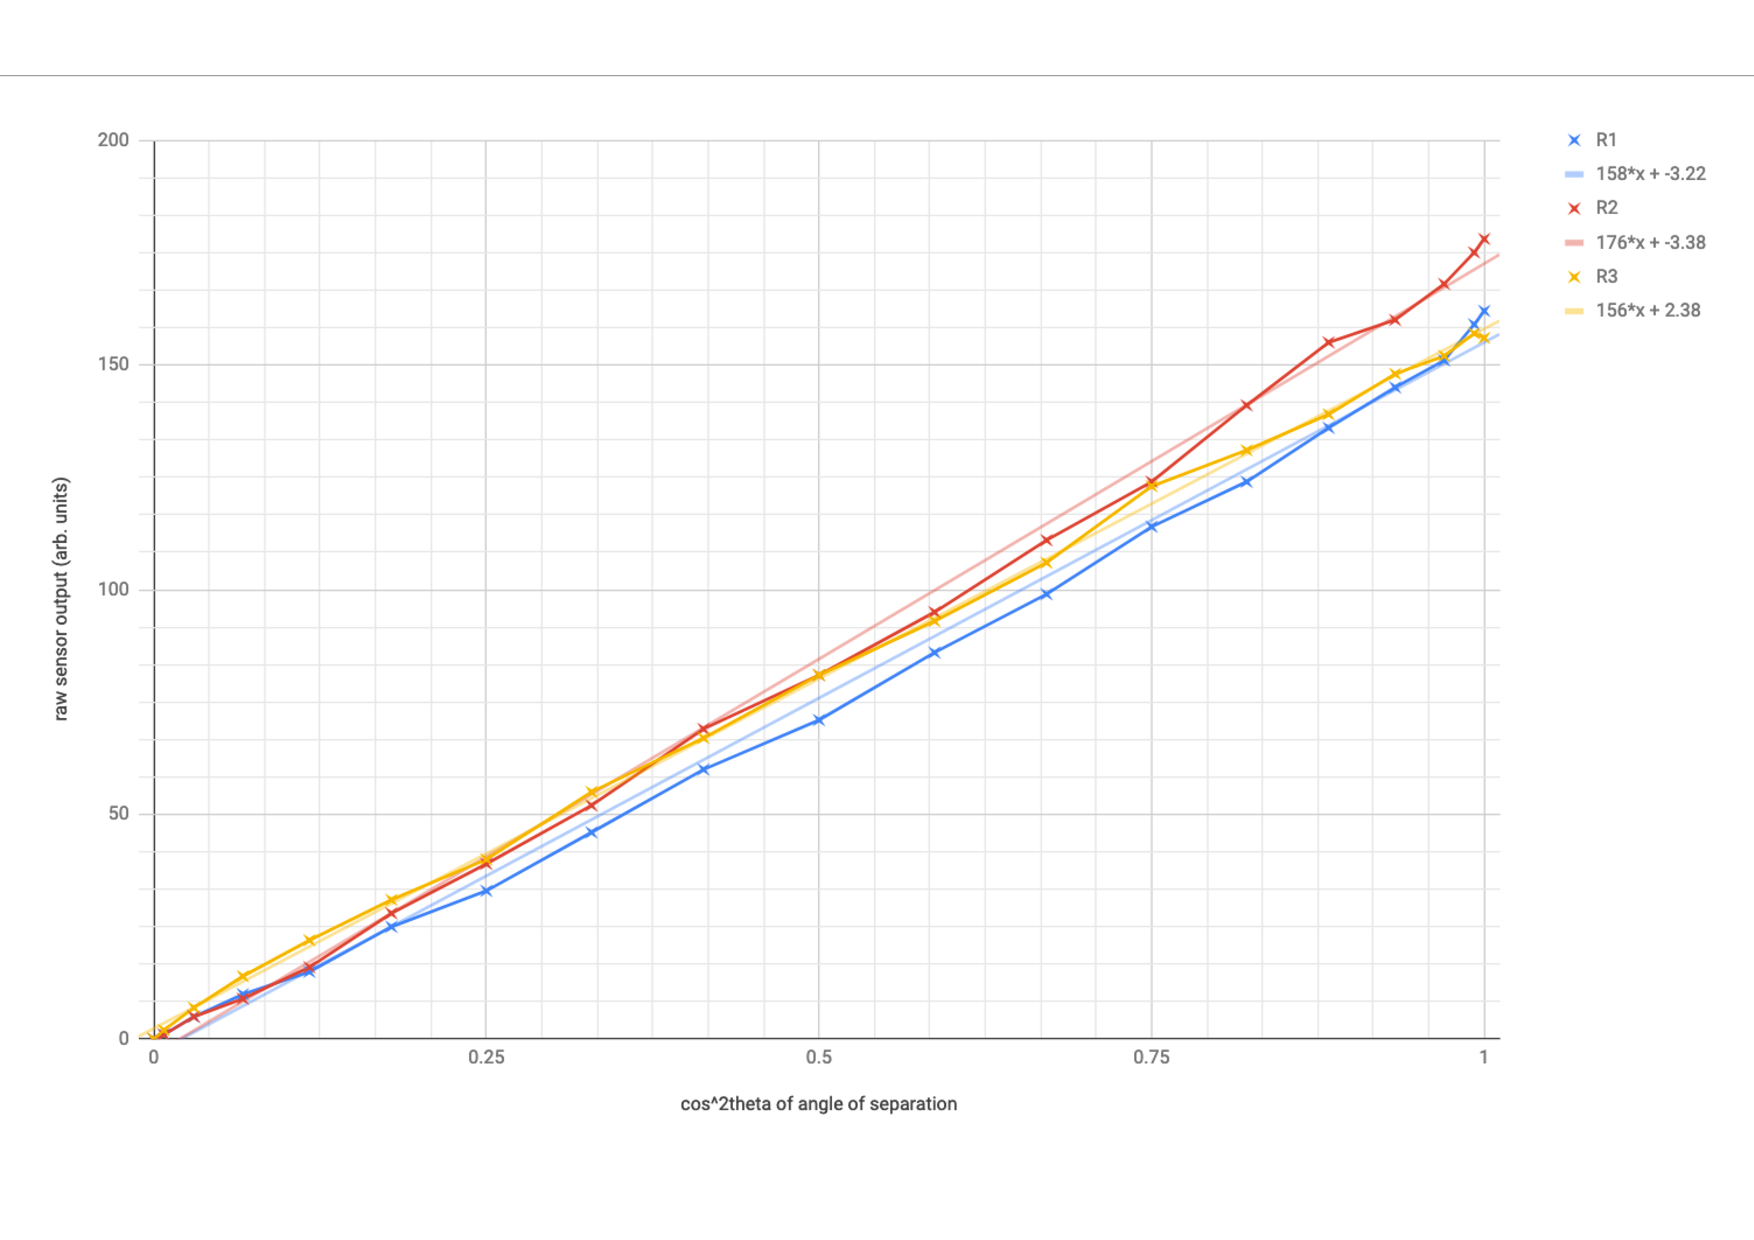
\includegraphics[keepaspectratio=true,width=\dimmin{}{\dimwidth{0.90}}]{images/green}{}\mdline{136}%mdk

%mdk-data-line={140}
\noindent\mdline{140}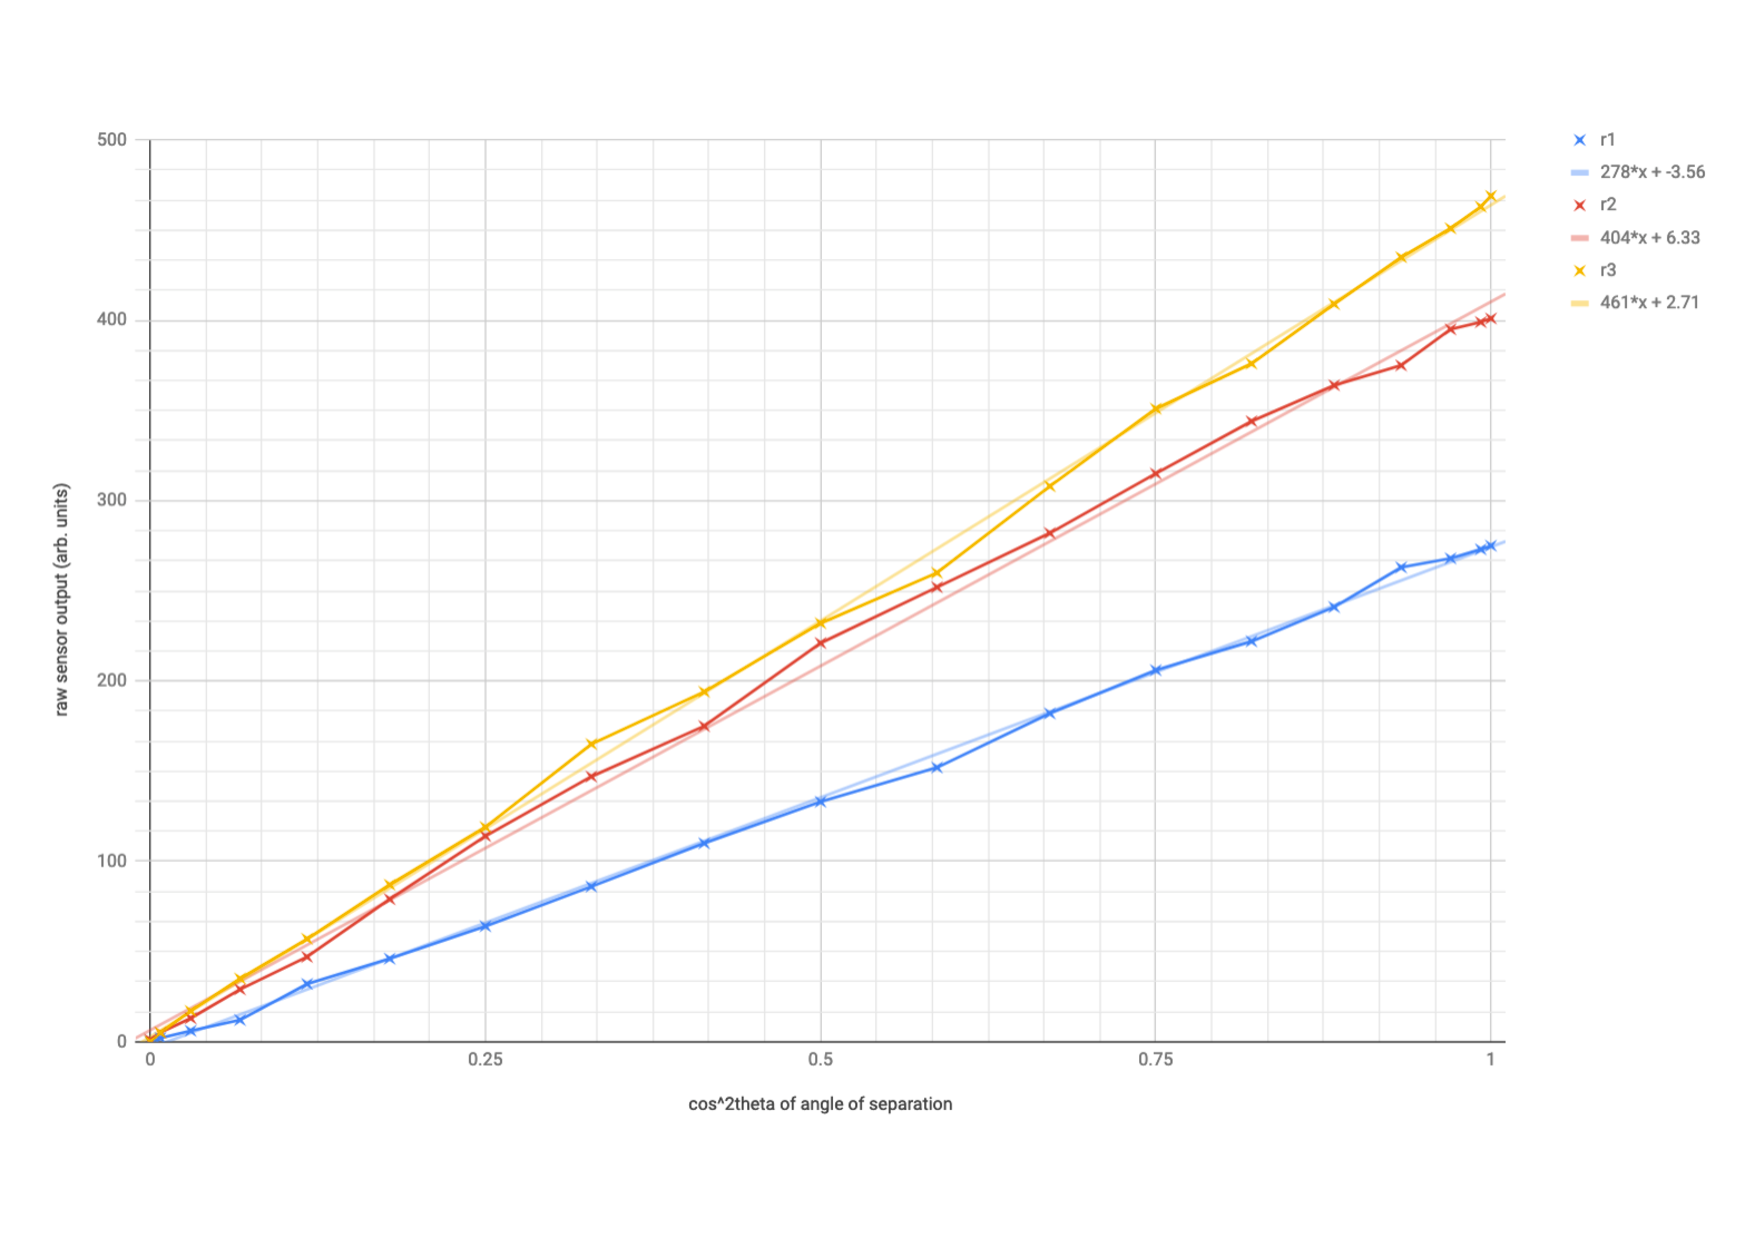
\includegraphics[keepaspectratio=true,width=\dimmin{}{\dimwidth{0.90}}]{images/blue}{}\mdline{140}%mdk

%mdk-data-line={144}
\noindent\mdline{144}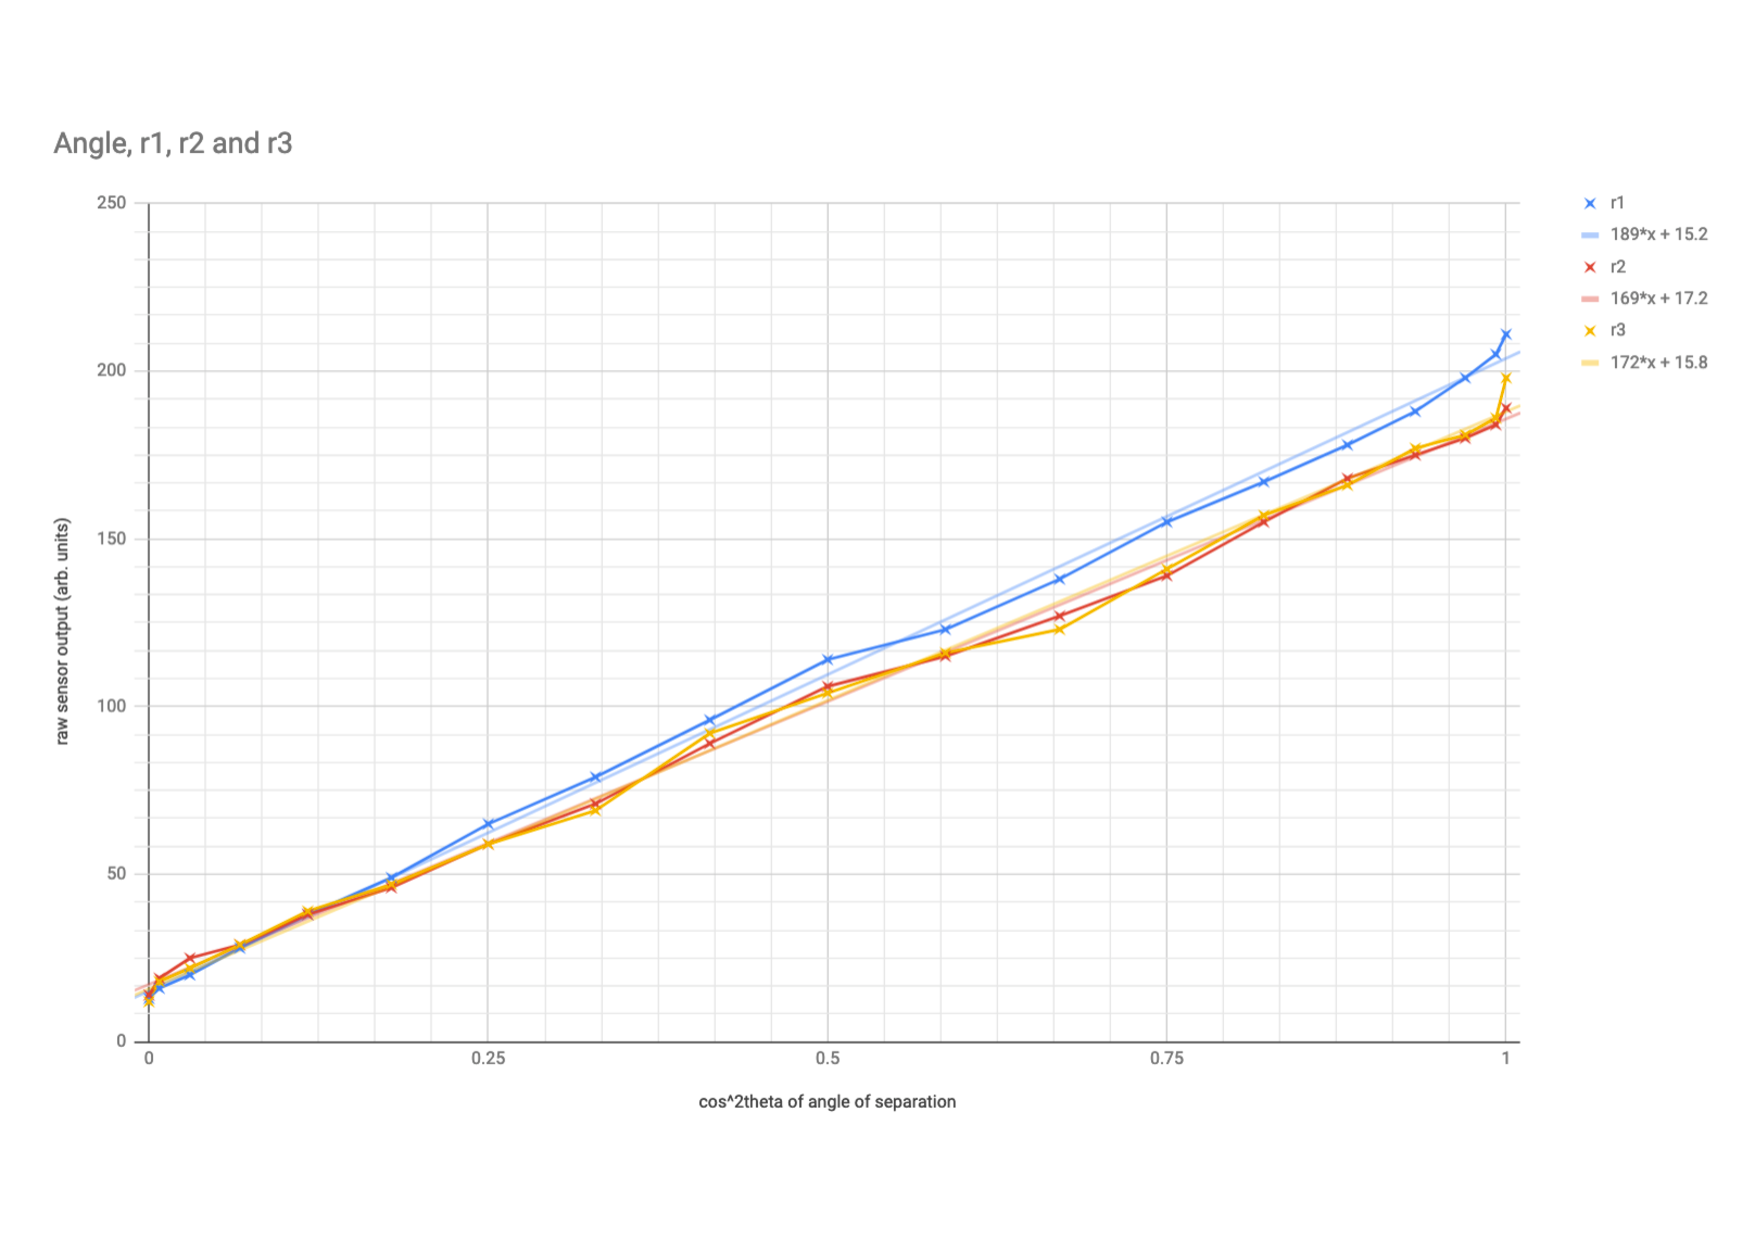
\includegraphics[keepaspectratio=true,width=\dimmin{}{\dimwidth{0.90}}]{images/red}{}\mdline{144}%mdk

%mdk-data-line={149}
\noindent\mdline{149}From these graphs, we can see that each repeat produces roughly the same result\mdline{149} \mdline{149}- the line of best fit produces gradients which are roughly equal to the initial intensity \mdline{149}$I_0$\mdline{149}. From this, combined with the accurate prediction of a linear function, shows with considerable confidence that these results experimentally verify Malus\mdline{149}'\mdline{149}s law.%mdk

%mdk-data-line={151}
\mdline{151}For each repeat, the calculated \mdline{151}$I_0$\mdline{151} is not exactly as observed, as seen in table\mdline{151}~\mdref{diff}{\mdcaptionlabel{4}}\mdline{151}%mdk

%mdk-data-line={153}
\begin{table}[H]%mdk
\begin{mdcenter}%mdk
\begin{mdtabular}{4}{\dimeval{(\linewidth)/4}}{1ex}%mdk
\begin{tabular}{lccc}\cmidrule[\dimpx{2}]{2-2}\cmidrule[\dimpx{2}]{3-3}\cmidrule[\dimpx{2}]{4-4}
{\mdseries\mdline{155}Repeat}&{\mdseries\mdline{155} Observed}&{\mdseries\mdline{155} Calculated}&{\mdseries\mdline{155} Difference}\\

\midrule
\mdline{157} 1&\mdline{157} 1240&\mdline{157} 1237&\mdline{157} 3\\
\mdline{158} 2&\mdline{158} 1121&\mdline{158} 1093&\mdline{158} 28\\
\mdline{159} 3&\mdline{159} 1255&\mdline{159} 1226&\mdline{159} 29\\
\midrule[\dimpx{2}]
\end{tabular}\end{mdtabular}

%mdk-data-line={162}
\mdhr{}%mdk

%mdk-data-line={163}
\noindent\mdline{163}\mdcaption{\textbf{Table~\mdcaptionlabel{4}.}~\mdcaptiontext{Difference in observed and calculated $I_0$}}%mdk
%mdk
\end{mdcenter}\label{diff}%mdk
%mdk
\end{table}%mdk

%mdk-data-line={165}
\mdline{165}This shows differences between observed and calculated initial intensities within acceptable error ranges. The difference can mostly be explained by the neutral density effect of the polarising filters\mdline{165} \mdline{165}- even at zero degrees there is a significant reduction in intensity with and without the filter.%mdk

%mdk-data-line={167}
\mdline{167}These results also seem to indicate that the original method (with two separate clamp stands for each filter) seemed to produce more accurate results than the secondary method (with one clamp stand for both filters sandwiched together). However, repeats two and three clearly show a better line of best fit, with much larger deviation from best fit in repeat one. This means that the accuracy is purely a coincidentally better gradient.%mdk%mdk


\end{document}
